
\documentclass[8pt]{beamer}
\usepackage{graphicx}                       % loads images
\usepackage{color}                          % for color in text
\usepackage{float}                          % to place [H]
\usepackage{amsmath}
\usepackage{amssymb}
\usepackage{bbm}
\usepackage{booktabs}
\usepackage{longtable}
\usepackage{bigstrut}
\usepackage{array}

    
\usepackage{tikz}
\usetikzlibrary{shapes.geometric, arrows}
\usepackage{multirow}
\usepackage{xr}
%\usepackage[round]{natbib}



% \usepackage[backend=biber, style=alphabetic ,
% citestyle=authoryear]{biblatex}
%   % biber is version 2.4; the latest?


% \addbibresource{../paper/References.bib}




\graphicspath{{../pilot_3/Figuras/}}
\usepackage{color}
%\usepackage{morefloats}
%\usepackage{showkeys}

\usepackage{enumerate}
\usepackage[labelfont=bf]{caption}
\usepackage[labelfont=bf, justification=justified]{subcaption}
\captionsetup{position=top}
\captionsetup[subfigure]{justification=centering}



\usepackage{epstopdf}
\epstopdfDeclareGraphicsRule{.tiff}{png}{.png}{convert #1 \OutputFile}
\AppendGraphicsExtensions{.tiff}


\usepackage{setspace}

\renewcommand{\rmdefault}{ppl}
\definecolor{darkred}{rgb}{0.8, 0.0, 0.0}
\definecolor{navyblue}{rgb}{0.0, 0.0, 0.8}
\definecolor{cadmiumgreen}{rgb}{0.0, 0.6, 0.24}

\usepackage{hyperref}
\hypersetup{
    pdfstartview={FitH},    		% fits the width of the page to the window
    pdftitle={Pilot 3},    % title
    pdfauthor={IML},     % author
    colorlinks=true,       % false: boxed links; true: colored links
    linkcolor=black,          % color of internal links (change box color with linkbordercolor)
    citecolor=darkred,        % color of links to bibliography
    filecolor=magenta,      % color of file links
    urlcolor=darkred           % color of external links
}

\newcommand{\green}[1]{\textcolor{cadmiumgreen}{#1}}

\newcommand{\comment}[1]
{\par {\bfseries \color{blue} #1 \par}}
%\usepackage{showkeys}
\setbeamertemplate{theorems}[numbered]
\newtheorem{claim}[theorem]{Claim}


% There are many different themes available for Beamer. A comprehensive
% list with examples is given here:
% http://deic.uab.es/~iblanes/beamer_gallery/index_by_theme.html
% You can uncomment the themes below if you would like to use a different
% one:
%\usetheme{AnnArbor}
%\usetheme{Antibes}
%\usetheme{Bergen}
%\usetheme{Berkeley}
%\usetheme{Berlin}
%\usetheme{Boadilla}
%\usetheme{boxes}
%\usetheme{CambridgeUS}
%\usetheme{Copenhagen}
%\usetheme{Darmstadt}
%\usetheme{default}
%\usetheme{Frankfurt}
%\usetheme{Goettingen}
%\usetheme{Hannover}
%\usetheme{Ilmenau}
%\usetheme{JuanLesPins}
%\usetheme{Luebeck}
\usetheme{Madrid}
%\usetheme{Malmoe}
%\usetheme{Marburg}
%\usetheme{Montpellier}
%\usetheme{PaloAlto}
%\usetheme{Pittsburgh}
%\usetheme{Rochester}
%\usetheme{Singapore}
%\usetheme{Szeged}
%\usetheme{Warsaw}

\setbeamertemplate{headline}{%
    \leavevmode%
    \hbox{%
        \begin{beamercolorbox}[wd=\paperwidth,ht=2.5ex,dp=1.125ex]{palette quaternary}%
            \insertsectionnavigationhorizontal{\paperwidth}{}{\hskip0pt plus1filll}
        \end{beamercolorbox}%
    }
}
\setbeamercovered{invisible}
\title{Something about lawyer quality, agency, and labor court outcomes }

% A subtitle is optional and this may be deleted
\subtitle{Subtitle}

\author{J. Sadka\inst{1} \and E. Seira\inst{2} \and C. Woodruff\inst{3}}
% - Give the names in the same order as the appear in the paper.
% - Use the \inst{?} command only if the authors have different
%   affiliation.

\institute[ITAM, Oxford] % (optional, but mostly needed)
{
  \inst{1,2}%
  ITAM
  \and
  \inst{3}%
  Oxford
}
% - Use the \inst command only if there are several affiliations.
% - Keep it simple, no one is interested in your street address.

\date{Fall 2018}
% - Either use conference name or its abbreviation.
% - Not really informative to the audience, more for people (including
%   yourself) who are reading the slides online

\subject{Applied Microeconomics}
% This is only inserted into the PDF information catalog. Can be left
% out. 

% If you have a file called "university-logo-filename.xxx", where xxx
% is a graphic format that can be processed by latex or pdflatex,
% resp., then you can add a logo as follows:

% \pgfdeclareimage[height=0.5cm]{university-logo}{university-logo-filename}
% \logo{\pgfuseimage{university-logo}}

% Delete this, if you do not want the table of contents to pop up at
% the beginning of each subsection:

% Let's get started
\begin{document}

\begin{frame}
  \titlepage
\end{frame}

\section*{Outline}
\begin{frame}{Outline}
\tableofcontents
\end{frame}

%%%%%%%%%%%%%%%%%%%%%%%%%%%%%%%%%%%%%%%%%%%%%%%%%%%%%%%%%%%%%%%%%%%%%%%%%%%
\section{Sketch of project}
\begin{frame}{Sketch of project}
\begin{itemize}
    \item Previous work with Mexico City Labor Court found:
    \begin{enumerate}
        \item Providing information on predicted case outcomes increases settlement rates
        \item Only when the plaintiff is present to receive the information...
        \item ...even over time
        \item Effect is of comparable magnitude to inducing conversation with a conciliator
    \end{enumerate}
\end{itemize}

RCT with cases already filed

\end{frame}


\begin{frame}{Previous results}

\begin{table}[H]
    \caption{Treatment Effects}
    \label{Treatment_effects}
    \begin{center}
    \scriptsize{% Table generated by Excel2LaTeX from sheet 'treatment_effects'
\begin{tabular}{lccccccccc}
\toprule
\multicolumn{1}{|r}{} & \multicolumn{9}{c}{Months after treatment} \\
\midrule
\multicolumn{1}{r|}{} & \multicolumn{5}{c|}{Same day settlement} & \multicolumn{1}{c|}{2 months } & \multicolumn{1}{c|}{ 5 months} & \multicolumn{1}{c|}{Long run} & Same day  \\
\midrule
\midrule
\multicolumn{1}{r|}{} & \multicolumn{2}{c|}{Phase 1} & \multicolumn{2}{c|}{Phase 2} & \multicolumn{5}{c}{Phase 1/2} \\
\midrule
\multicolumn{1}{r|}{} & \multicolumn{5}{c|}{OLS}              & \multicolumn{3}{c|}{OLS} & CF OLS \\
\midrule
\midrule
      & (1)   & (2)   & (3)   & (4)   & (5)   & (6)   & (7)   & (8)   & (9) \\
\midrule
\midrule
Control (constant) & 0.060*** & 0.034*** & 0.11*** & 0.10*** & 0.094*** & 0.15*** & 0.39*** & 0.45*** & 0.053 \\
      & (0.013) & (0.011) & (0.030) & (0.030) & (0.026) & (0.043) & (0.039) & (0.049) & (0.039) \\
Calculator & 0.051** & 0.019 & 0.047** & 0.0077 & 0.018 & 0.0035 & -0.0069 & -0.0025 & 0.0084 \\
      & (0.022) & (0.019) & (0.021) & (0.019) & (0.014) & (0.021) & (0.024) & (0.025) & (0.015) \\
Emp present (EP) &       & 0.14*** &       & 0.14* & 0.14*** & 0.11** & 0.094* & 0.070 & 0.47** \\
      &       & (0.050) &       & (0.072) & (0.041) & (0.046) & (0.048) & (0.050) & (0.21) \\
Calculator\#EP &       & 0.16** &       & 0.16* & 0.16*** & 0.18*** & 0.16** & 0.14** & 0.16*** \\
      &       & (0.079) &       & (0.089) & (0.056) & (0.061) & (0.064) & (0.061) & (0.056) \\
Control Function &       &       &       &       &       &       &       &       & -0.19 \\
      &       &       &       &       &       &       &       &       & (0.12) \\
      &       &       &       &       &       &       &       &       &  \\
\midrule
Observations & 1074  & 1074  & 1092  & 1092  & 2166  & 2166  & 2166  & 2166  & 2166 \\
R-squared & 0.0072 & 0.12  & 0.051 & 0.11  & 0.13  & 0.12  & 0.11  & 0.087 & 0.135 \\
Court dummies  & NO    & NO    & YES   & YES   & YES   & YES   & YES   & YES   & YES \\
DepVarMean & \multicolumn{2}{c}{0.095} & \multicolumn{2}{c}{0.20} & 0.15  & 0.19  & 0.32  & 0.43  & 0.15 \\
InteractionVarMean &       & 0.18  &       & \multicolumn{6}{c}{0.18} \\
\bottomrule
\bottomrule
\end{tabular}%
}
    \end{center}
\end{table}


\end{frame}

\begin{frame}{Sketch of project}
\begin{itemize}
    \item Was an RCT with live cases already filed in the court
   \item Suggests there may be agency issues with lawyers
  \item But lawyers are not randomly assigned, and we have no measure of quality
\end{itemize}

This project: Intervene as the fired workers approach the court, before they have a lawyer
 \end{frame}
 
 \begin{frame}{Intervention}

\begin{figure}[H]
    \caption{Information booth}
    \begin{center}
    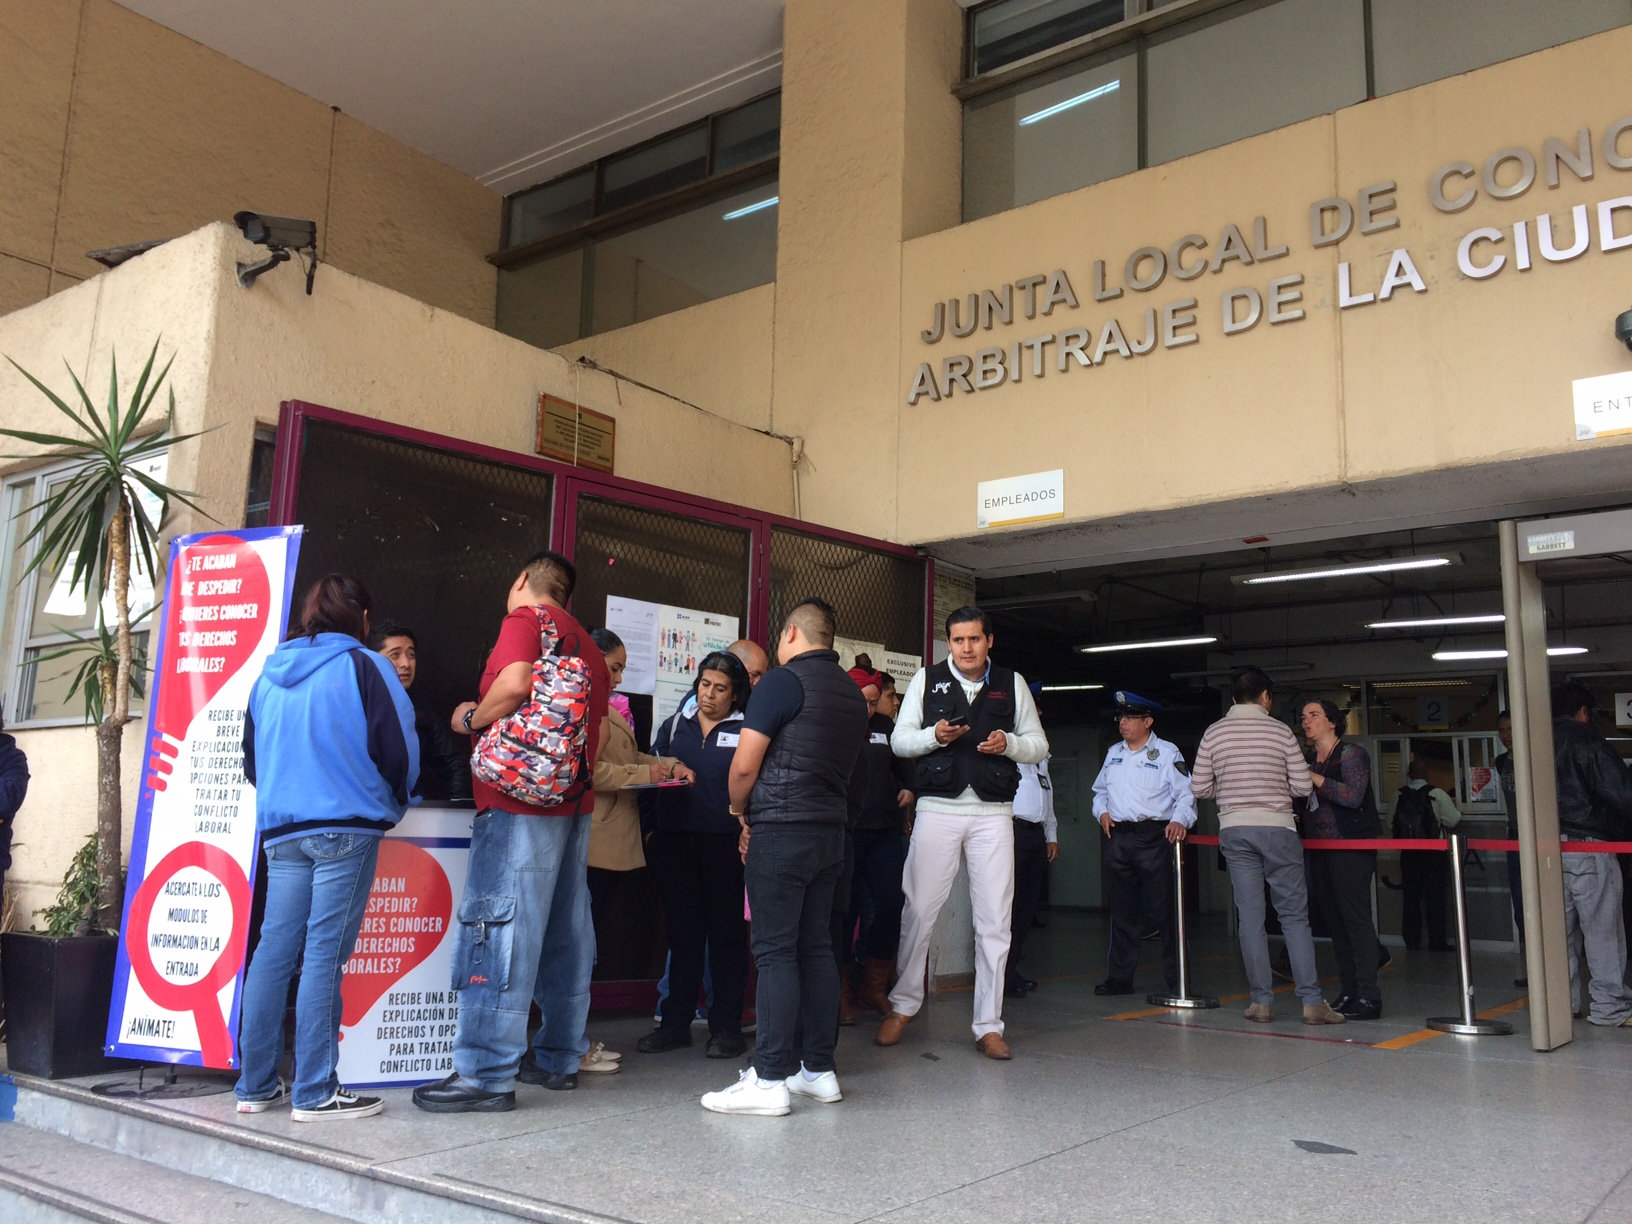
\includegraphics[width=1\textwidth]{presentations/IMG_1437.jpg}
    \end{center}
\end{figure}
\end{frame}

\begin{frame}{Interventions}
RCT with treatment randomized by day
\begin{enumerate}
    \item Court information (control, but no longer pure control)
    \item Uber ride to public attorney's office
    \begin{itemize}
        \item Adapted design following Sept 2017 earthquake
    \end{itemize}
    \item Calculator 
    \item Calculator + appointment letter for conciliator meeting
\end{enumerate}
Outcomes of in\begin{itemize}
    \item Do they settle or sue?
    \item Do they use public or private lawyer?
    \item If private lawyer, do they choose a higher-quality private lawyer?
    \item Characteristics of the case
    \item Measures of well-being (phone survey)
\end{itemize}
\end{frame}
 
 \begin{frame}{Goal for today}
What I'd like feedback on. First, two channels: \\
\vspace{.1in}
 Treatment \xrightarrow{} $Selection of lawyer$ \xrightarrow{} $outcome of case?$  \\
 
 \pause \\
 \vspace{.1in}
 Or:
 \\
 \vspace{.1in}
    Treatment \xrightarrow{} $Change in expectations$ \xrightarrow{} $(selection of lawyer)$ \xrightarrow{} $outcome of case$

    \pause
    \vspace{.2in}
\begin{itemize}
\item Some key outcomes are measured only if the plaintiff pursues a suit (i.e., does not settle or drop prior to filing)
\item The initial treatments have an effect on whether the case is filed or not
\item How much can we say about the outcomes conditional on filing? 
\end{itemize}

\end{frame}




%%%%%%%%%%%%%%%%%%%%%%%%%%%%%%%%%%%%%%%%%%%%%%%%%%%%%%%%%%%%%%%%%%%%%%%%%%%
\section{Summary statistics}

\begin{frame}{Summary statistics}
    \begin{table}[H]
\caption{SS}
\begin{center}
\tiny{% Table generated by Excel2LaTeX from sheet 'SS'
\begin{tabular}{lccc}
\toprule
Variable & \multicolumn{3}{c}{Treatment} \\
\midrule
\midrule
      & T1    & T2    & T3 \\
\midrule
      & \multicolumn{3}{c}{Admin data} \\
\midrule
\midrule
Female & 0.45  & 0.46  & 0.45 \\
      & (0.02) & (0.02) & (0.02) \\
Daily wage & 352.05 & 293.51 & 312.07 \\
      & (26.87) & (8.54) & (15.24) \\
Tenure & 3.65  & 3.73  & 3.67 \\
      & (0.16) & (0.15) & (0.19) \\
\midrule
      & \multicolumn{3}{c}{Expectations (Baseline)} \\
\midrule
\midrule
Prob winning & 0.89  & 0.87  & 0.89 \\
      & (0.01) & (0.01) & (0.01) \\
Prob winning above mean & 0.84  & 0.8   & 0.83 \\
      & (0.01) & (0.01) & (0.02) \\
Amt winning & 56126 & 60107 & 60853 \\
      & (3442) & (3901) & (5020) \\
Amt winning above mean & 0.47  & 0.48  & 0.45 \\
      & (0.02) & (0.02) & (0.02) \\
\midrule
Observations & 995   & 914   & 624 \\
\midrule
      & \multicolumn{3}{c}{Main outcomes} \\
\midrule
\midrule
Talked to lawyer & 0.61  & 0.6   & 0.41 \\
      & (0.02) & (0.02) & (0.02) \\
Solved conflict & 0.51  & 0.56  & 0.67 \\
      & (0.02) & (0.02) & (0.02) \\
Sued  & 0.4   & 0.34  & 0.28 \\
      & (0.02) & (0.02) & (0.02) \\
Sued w/public & 0.52  & 0.44  & 0.56 \\
      & (0.03) & (0.03) & (0.04) \\
\midrule
Observations & 661   & 598   & 385 \\
\bottomrule
\bottomrule
\end{tabular}%
}
\end{center}
 \footnotesize
\textit{Notes:} Summary statistics of main variables. Standard errors are shown in parenthesis.   
\textit{Do file: } \texttt{SS.do}
\end{table}
\end{frame}

%\begin{frame}{Summary statistics : A/B}
%    \begin{table}[H]
%\caption{SS :  A/B}
%\begin{center}
%\tiny{% Table generated by Excel2LaTeX from sheet 'SS'
\begin{tabular}{lcc}
\toprule
Variable & \multicolumn{2}{c}{Treatment} \\
\midrule
\midrule
      & A     & B \\
\midrule
      & \multicolumn{2}{c}{Admin data} \\
\midrule
\midrule
Female & 0.47  & 0.45 \\
      & (0.02) & (0.02) \\
Daily wage & 346.47 & 323.87 \\
      & (24.58) & (14.43) \\
Tenure & 3.7   & 3.9 \\
      & (0.15) & (0.21) \\
\midrule
      & \multicolumn{2}{c}{Expectations (Baseline)} \\
\midrule
\midrule
Prob winning & 0.87  & 0.9 \\
      & (0.01) & (0.01) \\
Prob winning above mean & 0.81  & 0.88 \\
      & (0.01) & (0.01) \\
Amt winning & 53237 & 57994 \\
      & (3043) & (4196) \\
Amt winning above mean & 0.37  & 0.4 \\
      & (0.02) & (0.02) \\
\midrule
Observations & 883   & 685 \\
\midrule
      & \multicolumn{2}{c}{Main outcomes} \\
\midrule
\midrule
Talked to lawyer & 0.74  & 0.78 \\
      & (0.02) & (0.02) \\
Solved conflict & 0.52  & 0.54 \\
      & (0.02) & (0.02) \\
Sued  & 0.4   & 0.38 \\
      & (0.02) & (0.02) \\
Sued w/public & 0.5   & 0.67 \\
      & (0.03) & (0.03) \\
\midrule
Observations & 511   & 465 \\
\bottomrule
\bottomrule
\end{tabular}%
}
%\end{center}
% \footnotesize
%\textit{Notes:} Summary statistics of main variables. %Standard errors are shown in parenthesis.   
%\textit{Do file: } \texttt{SS.do}
%\end{table}
%\end{frame}


%%%%%%%%%%%%%%%%%%%%%%%%%%%%%%%%%%%%%%%%%%%%%%%%%%%%%%%%%%%%%%%%%%%%%%%%%%%
\section{Expectations}

\begin{frame}{Expectations}
    

\begin{figure}[H]
    \caption{Histograms of expectations}
    \label{hist_exp}
    \begin{center}
        \begin{subfigure}{0.45\textwidth}
            \caption{Amount}
            \centering
            \includegraphics[width=\textwidth]{hist_exp_amt.pdf}
        \end{subfigure}
        \begin{subfigure}{0.45\textwidth}
            \caption{Probability}
                \centering
                \includegraphics[width=\textwidth]{hist_exp_prob.pdf}
        \end{subfigure}
        \end{center}
        \end{figure}
\end{frame}


%%%%%%%%%%%%%%%%%%%%%%%%%%%%%%%%%%%%%%%%%%%%%%%%%%%%%%%%%%%%%%%%%%%%%%%%%%%


%%%%%%%%%%%%%%%%%%%%%%%%%%%%%%%%%%%%%%%%%%%%%%%%%%%%%%%%%%%%%%%%%%%%%%%%%%%
\section{Treatment effects}

\subsection{Main results}
\begin{frame}{Main results}

 \begin{table}[H] 
 \begin{subtable}{1.\textwidth}
 \begin{center}
 \tiny{% Table generated by Excel2LaTeX from sheet 'reg_main_treat_pres'
\begin{tabular}{lcccccc}
\toprule
      & Solved conflict & Talked to lawyer & Talked to public lawyer & Informal Lawyer & Sued  & Sued w/public \\
\midrule
\midrule
      & (1)   & (2)   & (3)   & (4)   & (5)   & (6) \\
\midrule
\midrule
Treatment 2 & 0.052* & -0.0070 & -0.19*** & -0.19*** & -0.060** & -0.082* \\
      & (0.028) & (0.028) & (0.038) & (0.053) & (0.027) & (0.046) \\
Treatment 3 & 0.16*** & -0.20*** & -0.34*** & -0.13** & -0.12*** & 0.043 \\
      & (0.033) & (0.032) & (0.048) & (0.066) & (0.031) & (0.058) \\
Constant  & 0.50*** & 0.60*** & 0.69*** & 0.47*** & 0.38*** & 0.51*** \\
      & (0.025) & (0.026) & (0.035) & (0.061) & (0.025) & (0.036) \\
      &       &       &       &       &       &  \\
\midrule
Observations & 2057  & 1814  & 1014  & 341   & 1991  & 676 \\
R-squared & 0.022 & 0.028 & 0.076 & 0.070 & 0.014 & 0.017 \\
T2=T3 & 0.00050 & 2.4e-09 & 0.0035 & 0.31  & 0.031 & 0.043 \\
BVC   & YES   & YES   & YES   & YES   & YES   & YES \\
Source & 2m    & 2w    & 2w    & 2m    & 2m    & 2m \\
Obs per group & 788/744/525 & 722/669/423 & 439/402/173 & 141/139/61 & 765/725/501 & 301/240/135 \\
Days per group & 93/106/75 & 81/91/61 & 79/88/57 & 66/71/37 & 93/106/75 & 84/88/60 \\
\bottomrule
\bottomrule
\end{tabular}%
}
 \end{center}
 \end{subtable}
 \end{table}  
 
\end{frame}

\begin{frame}{Lee bounds}

\begin{figure}[H]
    \caption{Lee Bounds}
    \label{lee_bounds}
    \begin{center}
        \begin{subfigure}{0.49\textwidth}
            \centering
            \includegraphics[width=\textwidth]{lee_bounds_2w.pdf}
        \end{subfigure}
        \begin{subfigure}{0.49\textwidth}
                \centering
                \includegraphics[width=\textwidth]{lee_bounds_2m.pdf}
        \end{subfigure}
    \end{center} 
\end{figure} 
 
\end{frame}

\subsection{Results of expectations}
\begin{frame}{Expectations for different arms}

\begin{figure}[H]
    \begin{center}
        \begin{subfigure}{0.49\textwidth}
            \centering
            \includegraphics[width=\textwidth]{lee_bounds_exp_amt.pdf}
        \end{subfigure}
        \begin{subfigure}{0.49\textwidth}
                \centering
                \includegraphics[width=\textwidth]{lee_bounds_exp_prob.pdf}
        \end{subfigure}
    \end{center} 
\end{figure} 
\end{frame}

\begin{frame}{Update of expectations}

\begin{figure}[H]
    \begin{center}
        \begin{subfigure}{0.49\textwidth}
            \centering
            \includegraphics[width=\textwidth]{lee_bounds_diff_amt.pdf}
        \end{subfigure}
        \begin{subfigure}{0.49\textwidth}
                \centering
                \includegraphics[width=\textwidth]{lee_bounds_diff_prob.pdf}
        \end{subfigure}
    \end{center} 
\end{figure} 
 
 
\end{frame}


\subsection{Updating as driver of the TE}
\begin{frame}{Updating as driver of the TE}
Now, to explore the impact of the update in expectations in the settlement rate, we perform a 2SLS instrumenting the immediate decrease in expectations with treatment.

\[\text{settlement}=\alpha_{IV}+\beta_{IV}\widetilde{\text{Decrease expectation}}+\gamma_{IV}X\]

\[\text{Decrease expectation}=\alpha_{FS}+\beta_{FS}\text{Treatment}+\gamma_{FS}X\]

where decrease expectations is either
\begin{enumerate}
    \item Dummy: $1(\text{immediate expectation}<\text{baseline})$
    \item Continuous: $\text{immediate expectation}-\text{baseline}$
\end{enumerate}
\end{frame}

\begin{frame}{Updating as driver of the TE}

\begin{table}[H]
\caption{Immediate updating in 2M settlement}
\begin{center}
\tiny{% Table generated by Excel2LaTeX from sheet 'iv_inm_update_2m'
\begin{tabular}{lllllllll}
      & \multicolumn{8}{c}{Settlement 2M} \\
\midrule
      & \multicolumn{4}{c}{Probability} & \multicolumn{4}{c}{Amount} \\
\midrule
\midrule
      & \multicolumn{2}{c}{Dummy} & \multicolumn{2}{c}{Continuous} & \multicolumn{2}{c}{Dummy} & \multicolumn{2}{c}{Continuous} \\
\midrule
      & 2S    & FS    & 2S    & FS    & 2S    & FS    & 2S    & FS \\
\midrule
\midrule
      & (1)   & (2)   & (3)   & (4)   & (5)   & (6)   & (7)   & (8) \\
\midrule
\midrule
Decrease exp & 0.25*** &       & -1.17** &       & 0.45*** &       & 0.000017 &  \\
      & (0.095) &       & (0.49) &       & (0.16) &       & (0.000020) &  \\
Treatment 1  &       & 0.0064 &       & -0.0051 &       & -0.0052 &       & -2995.6 \\
      &       & (0.0099) &       & (0.0037) &       & (0.014) &       & (8351.5) \\
Treatment 2 &       & 0.31*** &       & -0.061*** &       & 0.26*** &       & 3027.8 \\
      &       & (0.021) &       & (0.0077) &       & (0.028) &       & (3312.8) \\
Treatment 3 &       & 0.28*** &       & -0.053*** &       & 0.26*** &       & 10018.0 \\
      &       & (0.024) &       & (0.0091) &       & (0.034) &       & (11072.5) \\
Constant & 0.50*** &       & 0.50*** &       & 0.52*** &       & 0.58*** &  \\
      & (0.028) &       & (0.029) &       & (0.037) &       & (0.12) &  \\
      &       &       &       &       &       &       &       &  \\
\midrule
Observations & 1690  & 1690  & 1690  & 1690  & 779   & 779   & 779   & 779 \\
R-squared & 0.0026 & 0.14  & .     & 0.046 & .     & 0.13  & .     & 0.017 \\
BVC   & YES   & YES   & YES   & YES   & YES   & YES   & YES   & YES \\
Source & 2m    & 2m    & 2m    & 2m    & 2m    & 2m    & 2m    & 2m \\
\bottomrule
\bottomrule
\end{tabular}%
}
\end{center}
\end{table}     
\end{frame}

%%%%%%%%%%%%%%%%%%%%%%%%%%%%%%%%%%%%%%%%%%%%%%%%%%%%%%%%%%%%%%%%%%%%%%%%%%%
\section{Lawyers}

\begin{frame}{Lawyers on expectations}
    Now we focus on expectations and the role of private/public lawyers in expectations. 
\[\text{Survey expectation}= \alpha+\beta_11(\text{Public Lawyer}) + \beta_2 \text{Baseline} + \gamma X\]
\begin{table}[H]
      \centering
        \tiny{% Table generated by Excel2LaTeX from sheet 'reg_expectation_2m_pres'
\begin{tabular}{lcccc}
\toprule
      & Amt. Expectation & Amt. More than mean & Prob. Expectation & Prob. More than mean \\
\midrule
\midrule
      & (1)   & (2)   & (3)   & (4) \\
\midrule
\midrule
Public Lawyer & -15440.6*** & -0.13*** & -0.028** & -0.061** \\
      & (5007.3) & (0.031) & (0.013) & (0.027) \\
Baseline    & 0.74*** & -0.016 & 0.37*** & 0.17*** \\
      & (0.23) & (0.033) & (0.053) & (0.063) \\
Constant & 3399.3 & 0.36*** & 0.53*** & 0.66*** \\
      & (6286.8) & (0.041) & (0.052) & (0.073) \\
      &       &       &       &  \\
\midrule
Observations & 349   & 941   & 809   & 953 \\
R-squared & 0.66  & 0.11  & 0.11  & 0.017 \\
DepVarMean & 56150.7 & 0.34  & 0.86  & 0.78 \\
BVC   & YES   & YES   & YES   & YES \\
Source & 2m    & 2m    & 2m    & 2m \\
\bottomrule
\bottomrule
\end{tabular}%
}
\end{table}

\end{frame}


\subsection{Welfare - Quality}
\begin{frame}{Lawyer's quality}

 \begin{table}[H] 
 \begin{subtable}{1.\textwidth}
 \begin{center}
 \tiny{% Table generated by Excel2LaTeX from sheet 'lawyerstype_info_reg'
\begin{tabular}{lcc}
\toprule
      & \multicolumn{2}{c}{Wants to change lawyer} \\
\midrule
\midrule
      & (1)   & (2) \\
\midrule
\midrule
T2/Private formal & -0.13*** & -0.14*** \\
      & (0.041) & (0.037) \\
T3/Private informal & -0.14*** & 0.17*** \\
      & (0.050) & (0.054) \\
Constant & 0.36*** & 0.27*** \\
      & (0.042) & (0.039) \\
      &       &  \\
\midrule
Observations & 461   & 742 \\
R-squared & 0.031 & 0.063 \\
DepVarMean & \multicolumn{2}{c}{0.23} \\
BVC   & YES   & YES \\
Source & 2m    & 2m \\
\bottomrule
\bottomrule
\end{tabular}%
}
 \end{center}
 \end{subtable}
 \end{table}  
 
\end{frame}


\begin{frame}{Lawyer's quality}

 \begin{table}[H] 
 \begin{subtable}{1.\textwidth}
 \begin{center}
 \tiny{% Table generated by Excel2LaTeX from sheet 'welfare_reg_lawyer_2m_pres'
\begin{tabular}{lcccccccc}
\toprule
      & Happiness (0-10) & Stop paying serv. & Lack of money & Work  & Better job & Looking job & Prob. finds job & Time spent \\
\midrule
\midrule
      & (1)   & (2)   & (3)   & (4)   & (5)   & (6)   & (7)   & (8) \\
\midrule
\midrule
Private Formal & 0.29* & -0.070** & -0.099*** & 0.039 & 0.018 & 0.018 & 4.27  & 0.83 \\
      & (0.15) & (0.033) & (0.031) & (0.034) & (0.054) & (0.033) & (2.81) & (0.73) \\
Private Informal & 0.16  & -0.0077 & 0.049 & 0.014 & 0.010 & 0.052 & 14.0*** & -1.18 \\
      & (0.20) & (0.043) & (0.045) & (0.045) & (0.078) & (0.046) & (3.14) & (1.09) \\
Woman & -0.42*** & 0.022 & 0.018 & -0.11*** & 0.033 & -0.067** & 0.43  & -0.47 \\
      & (0.14) & (0.028) & (0.028) & (0.033) & (0.051) & (0.029) & (2.54) & (0.66) \\
Tenure & -0.044*** & -0.0000035 & 0.00017 & -0.010*** & -0.023*** & -0.0048 & -0.26 & 0.080 \\
      & (0.016) & (0.0029) & (0.0035) & (0.0027) & (0.0067) & (0.0034) & (0.25) & (0.063) \\
Daily wage & 0.000013 & 0.0000092 & -0.000025 & -0.000014 & 0.000027 & -0.000045*** & -0.00013 & 0.00050 \\
      & (0.000095) & (0.000014) & (0.000034) & (0.000020) & (0.000030) & (0.000014) & (0.0058) & (0.00049) \\
Constant & 7.91*** & 0.70*** & 0.65*** & 0.48*** & 0.57*** & 0.88*** & 66.0*** & 19.6*** \\
      & (0.13) & (0.025) & (0.029) & (0.030) & (0.050) & (0.028) & (2.84) & (0.62) \\
      &       &       &       &       &       &       &       &  \\
\midrule
Observations & 1078  & 1086  & 1089  & 1090  & 433   & 655   & 488   & 1030 \\
R-squared & 0.020 & 0.0058 & 0.014 & 0.023 & 0.028 & 0.019 & 0.027 & 0.0072 \\
DepVarMean & 7.66  & 0.69  & 0.62  & 0.40  & 0.53  & 0.82  & 68.2  & 20.0 \\
BVC   & YES   & YES   & YES   & YES   & YES   & YES   & YES   & YES \\
Source & 2m    & 2m    & 2m    & 2m    & 2m    & 2m    & 2m    & 2m \\
\bottomrule
\bottomrule
\end{tabular}%
}
 \end{center}
 \end{subtable}
 \end{table}  
 
\end{frame}


\begin{frame}{Welfare}

 \begin{table}[H] 
 \begin{subtable}{1.\textwidth}
 \begin{center}
 \tiny{% Table generated by Excel2LaTeX from sheet 'welfare_reg_2m_pres'
\begin{tabular}{lcccccccc}
\toprule
      & Happiness (0-10) & Stop paying serv. & Lack of money & Work  & Better job & Looking job & Prob. finds job & Time spent \\
\midrule
\midrule
      & (1)   & (2)   & (3)   & (4)   & (5)   & (6)   & (7)   & (8) \\
\midrule
\midrule
Treatment 2 & 0.13  & -0.070*** & -0.068*** & 0.019 & 0.031 & -0.038 & -0.24 & 1.11* \\
      & (0.12) & (0.024) & (0.025) & (0.025) & (0.035) & (0.026) & (2.21) & (0.67) \\
Treatment 3 & 0.29** & -0.071** & -0.076** & 0.021 & 0.012 & -0.030 & 3.59  & -0.56 \\
      & (0.13) & (0.032) & (0.032) & (0.032) & (0.041) & (0.030) & (2.59) & (0.78) \\
Woman & -0.30*** & 0.042* & 0.038 & -0.15*** & 0.039 & -0.035 & -2.35 & -0.39 \\
      & (0.094) & (0.022) & (0.024) & (0.024) & (0.031) & (0.024) & (1.80) & (0.53) \\
Tenure & -0.025** & -0.0027 & -0.0020 & -0.0083*** & -0.021*** & -0.0073*** & -0.67*** & 0.093* \\
      & (0.011) & (0.0024) & (0.0024) & (0.0021) & (0.0036) & (0.0026) & (0.23) & (0.054) \\
Daily wage & 0.0000080 & -0.000030 & -0.000044 & -0.000015 & -0.0000010 & -0.000023 & 0.0078** & 0.0011** \\
      & (0.000070) & (0.000033) & (0.000039) & (0.000021) & (0.000039) & (0.000030) & (0.0037) & (0.00044) \\
Constant & 8.12*** & 0.60*** & 0.56*** & 0.56*** & 0.59*** & 0.90*** & 69.7*** & 16.5*** \\
      & (0.10) & (0.024) & (0.027) & (0.023) & (0.032) & (0.028) & (2.09) & (0.58) \\
      &       &       &       &       &       &       &       &  \\
\midrule
Observations & 1958  & 1974  & 1976  & 1974  & 929   & 1042  & 764   & 1773 \\
R-squared & 0.011 & 0.0081 & 0.0084 & 0.028 & 0.030 & 0.015 & 0.022 & 0.0084 \\
T2=T3 & 0.19  & 0.98  & 0.79  & 0.94  & 0.65  & 0.78  & 0.15  & 0.042 \\
DepVarMean & 8.02  & 0.55  & 0.51  & 0.47  & 0.55  & 0.82  & 69.4  & 17.3 \\
BVC   & YES   & YES   & YES   & YES   & YES   & YES   & YES   & YES \\
Source & 2m    & 2m    & 2m    & 2m    & 2m    & 2m    & 2m    & 2m \\
\bottomrule
\bottomrule
\end{tabular}%
}
 \end{center}
 \end{subtable}
 \end{table}  
 
\end{frame}


\begin{frame}{Lawyer's Quality}
    The coefficients for the FE offices in a regression against are shown in increasing order in the plot below.
    
    \begin{figure}[H]
    \begin{center}
        \begin{subfigure}{0.49\textwidth}
        \caption{Positive recovery}
            \centering
            \includegraphics[width=\textwidth]{betas_pos_rec.pdf}
        \end{subfigure}
        \begin{subfigure}{0.49\textwidth}
        \caption{Duration}
                \centering
                \includegraphics[width=\textwidth]{betas_duration.pdf}
        \end{subfigure}
    \end{center} 
\end{figure} 
\end{frame}

\begin{frame}{Lawyer quality}

Exercise the measure the quality of cases. Three steps:
\begin{enumerate}
    \item Two lawyers read case files and identified "variables" that define the quality of the case
    \begin{itemize}
        \item Is the defendants address and phone number provided?
        \item Are the details of the dismissal complete
    \end{itemize}
    \item (Independently) Assign 8 lawyers to rate the quality of 500 filings (each filing read by 2 lawyers). 
    \begin{itemize}
        \item Overall rating
        \incentivized predictions of outcomes
    \end{itemize}
    \item Machine learning of rating (quality) on case characteristics. Then use the coefficients that come from this exercise to predict quality of cases filed in our experimental sample. 
\end{enumerate}
\end{frame}

\section{Help!}
\begin{frame}{Issues}
    \begin{itemize}
        \item Incentives to talk with public lawyers? It's complicated...
        \pause
    \begin{itemize}
        \item We see a reduction in talking with lawyers
        \item Now with the Uber treatment, it looks like an increase in talking with the public lawyers
        \item But, maybe the \textit{coyotes} are now at the public attorney's office instead of the court?
        \end{itemize}
        \pause
    \item Maybe the quality of the lawyers, conditional on filing, is higher. But this is a selected sample, because the treatment affects filing rates.     \end{itemize}
    In the end, I guess the struggle here is what is the main outcome we are looking for: \\
    \vspace{.1in}
   Treatment \xrightarrow{} $Selection of lawyer$ \xrightarrow{} $outcome of case?$  \\
 
 \vspace{.1in}
    Treatment \xrightarrow{} $Change in expectations$ \xrightarrow{} $(selection of lawyer)$ \xrightarrow{} $outcome of case$
\end{frame}
%%%%%%%%%%%%%%%%%%%%%%%%%%%%%%%%%%%%%%%%%%%%%%%%%%%%%%%%%%%%%%%%%%%%%%%%%%%




%%%%%%%%%%%%%%%%%%%%%%%%%%%%%%%%%%%%%%%%%%%%%%%%%%%%%%%%%%%%%%%%%%%%%%%%%%%
\section{Appendix}

\begin{frame}{Appendix - Balance}
\begin{table}[H] 
 \begin{subtable}{1.\textwidth}
 \begin{center}
 \tiny{% Table generated by Excel2LaTeX from sheet 'reg_balance_2m'
\begin{tabular}{lccccccc}
\toprule
\multicolumn{8}{c}{Main Treatment} \\
\midrule
\midrule
      & Woman  & Daily wage & Tenure & Mon-Tue & Angry & +High-School & Prob \\
\midrule
\midrule
      & (1)   & (2)   & (3)   & (4)   & (5)   & (6)   & (7) \\
\midrule
Treatment 2 & -0.0048 & -37.9 & 0.30  & 0.056 & 0.013 & 0.032 & -0.015 \\
      & (0.027) & (26.9) & (0.25) & (0.080) & (0.024) & (0.028) & (0.011) \\
Treatment 3 & 0.00029 & -37.7 & 0.19  & 0.0084 & 0.0051 & 0.010 & 0.0062 \\
      & (0.027) & (26.7) & (0.30) & (0.087) & (0.031) & (0.032) & (0.011) \\
Constant  & 0.46*** & 336.5*** & 3.42*** & 0.41*** & 0.76*** & 0.67*** & 0.89*** \\
      & (0.018) & (24.8) & (0.18) & (0.058) & (0.016) & (0.020) & (0.0075) \\
      &       &       &       &       &       &       &  \\
\midrule
Observations & 2057  & 2059  & 2059  & 2059  & 1983  & 1915  & 1793 \\
R-squared & 0.000022 & 0.0015 & 0.00080 & 0.0027 & 0.00018 & 0.00094 & 0.0029 \\
T2=T3 & 0.85  & 0.99  & 0.71  & 0.57  & 0.80  & 0.49  & 0.058 \\
Obs per group & 788/744/525 & 789/745/525 & 789/745/525 & 789/745/525 & 724/735/524 & 646/744/525 & 664/666/463 \\
\midrule
\midrule
      &       &       &       &       &       &       &  \\
      & NA prob & Prob above & NA prob above & Amt   & NA amt & Amt above & NA amt above \\
\midrule
\midrule
      & (8)   & (9)   & (10)  & (11)  & (12)  & (13)  & (14) \\
\midrule
Treatment 2 & -0.052** & -0.031 & -0.026 & 6428.5 & -0.029 & 0.028 & -0.024 \\
      & (0.020) & (0.023) & (0.020) & (5231.0) & (0.026) & (0.035) & (0.033) \\
Treatment 3 & -0.040* & 0.012 & -0.0055 & 5135.3 & -0.075** & -0.0046 & -0.018 \\
      & (0.022) & (0.022) & (0.021) & (6432.9) & (0.034) & (0.039) & (0.036) \\
Constant  & 0.16*** & 0.84*** & 0.11*** & 53597.9*** & 0.60*** & 0.46*** & 0.35*** \\
      & (0.016) & (0.015) & (0.015) & (3045.9) & (0.018) & (0.024) & (0.022) \\
      &       &       &       &       &       &       &  \\
\midrule
Observations & 2059  & 1862  & 2059  & 883   & 2059  & 1371  & 2059 \\
R-squared & 0.0049 & 0.0022 & 0.0016 & 0.0016 & 0.0035 & 0.00084 & 0.00051 \\
T2=T3 & 0.55  & 0.069 & 0.29  & 0.86  & 0.18  & 0.42  & 0.87 \\
Obs per group & 789/745/525 & 705/685/472 & 789/745/525 & 315/319/249 & 789/745/525 & 515/504/352 & 789/745/525 \\
\bottomrule
\bottomrule
\end{tabular}%
}
 \end{center}
 \end{subtable}
 \end{table}  
\end{frame}

\begin{frame}{Appendix - Updating}
    \begin{figure}[H]
    \caption{Immediate updating}
    \label{update_expimm}
    \begin{center}
        \begin{subfigure}{0.45\textwidth}
            \caption{Amount}
            \centering
            \includegraphics[width=\textwidth]{imm_exp_amt_nocond.pdf}
        \end{subfigure}
        \begin{subfigure}{0.45\textwidth}
            \caption{Probability}
                \centering
                \includegraphics[width=\textwidth]{imm_exp_prob_nocond.pdf}
        \end{subfigure}
    \end{center} 
         \scriptsize \textit{Notes:} Amount variables are trimmed at the 95th percentile.
\end{figure}
\end{frame}

\begin{frame}{Appendix - Updating}
        \begin{figure}[H]
    \caption{Updating at 2 weeks}
    \label{update_exp2w}
    \begin{center}
        \begin{subfigure}{0.45\textwidth}
            \caption{Amount}
            \centering
            \includegraphics[width=\textwidth]{2w_exp_amt_nocond.pdf}
        \end{subfigure}
        \begin{subfigure}{0.45\textwidth}
            \caption{Probability}
            \centering
            \includegraphics[width=\textwidth]{2w_exp_prob_nocond.pdf}
        \end{subfigure}
      \end{center} 
         \scriptsize \textit{Notes:} Amount variables are trimmed at the 95th percentile.
\end{figure}      
        
\end{frame}


\begin{frame}{Appendix - Updating}
    \begin{figure}[H]
    \caption{Updating at 2 months}
    \label{update_exp2m}
    \begin{center}
            \begin{subfigure}{0.45\textwidth}
            \caption{Amount}
            \centering
            \includegraphics[width=\textwidth]{2m_exp_amt_nocond.pdf}
        \end{subfigure}
        \begin{subfigure}{0.45\textwidth}
            \caption{Probability}
            \centering
            \includegraphics[width=\textwidth]{2m_exp_prob_nocond.pdf}
        \end{subfigure}
    \end{center} 
         \scriptsize \textit{Notes:} Amount variables are trimmed at the 95th percentile.
\end{figure}

\end{frame}


\begin{frame}{Appendix - Lee bounds ratio}
\begin{figure}[H]
    \begin{center}
        \begin{subfigure}{0.49\textwidth}
            \centering
            \includegraphics[width=\textwidth]{lee_bounds_ratio_amt.pdf}
        \end{subfigure}
        \begin{subfigure}{0.49\textwidth}
                \centering
                \includegraphics[width=\textwidth]{lee_bounds_ratio_prob.pdf}
        \end{subfigure}
    \end{center} 
\end{figure} 
 
 
\end{frame}


\begin{frame}{Appendix - Expectation at 2w}
\begin{table}[H]
      \centering
        \tiny{% Table generated by Excel2LaTeX from sheet 'reg_expectation_2w_pres'
\begin{tabular}{lcccc}
\toprule
      & Amt. Expectation & Amt. More than mean & Prob. Expectation & Prob. More than mean \\
\midrule
\midrule
      & (1)   & (2)   & (3)   & (4) \\
\midrule
\midrule
Public Lawyer & -9472.5* & -0.11*** & -0.0039 & 0.00041 \\
      & (5227.3) & (0.028) & (0.010) & (0.023) \\
Baseline amt   & 0.61*** & -0.062** & 0.46*** & 0.10** \\
      & (0.17) & (0.027) & (0.048) & (0.046) \\
Constant & 19320.3** & 0.37*** & 0.45*** & 0.72*** \\
      & (9000.5) & (0.037) & (0.045) & (0.050) \\
      &       &       &       &  \\
\midrule
Observations & 523   & 1265  & 1095  & 1339 \\
R-squared & 0.48  & 0.18  & 0.15  & 0.0092 \\
DepVarMean & 52184.9 & 0.35  & 0.87  & 0.82 \\
BVC   & YES   & YES   & YES   & YES \\
Source & 2w    & 2w    & 2w    & 2w \\
\bottomrule
\bottomrule
\end{tabular}%
}
\end{table}
\end{frame}

\begin{frame}{Appendix - Expectation by lawyer}
\begin{figure}[H]
    \caption{Linear polynomial smoothing of expectations by type of lawyer}
    \label{lps_type_law}
    \begin{center}
        \begin{subfigure}{0.45\textwidth}
            \caption{Amount}
            \centering
            \includegraphics[width=\textwidth]{lpoly_exp_amt_lawyer.pdf}
        \end{subfigure}
        \hfill
        \begin{subfigure}{0.45\textwidth}
            \caption{Probability}
                \centering
                \includegraphics[width=\textwidth]{lpoly_exp_prob_lawyer.pdf}
        \end{subfigure}
    \end{center} 
\end{figure}
\end{frame}

\begin{frame}{Appendix - Update \& settlement}
    
\begin{table}[H]
\caption{Immediate updating in 2W settlement}
\begin{center}
\tiny{% Table generated by Excel2LaTeX from sheet 'iv_inm_update_2w'
\begin{tabular}{lllllllll}
      & \multicolumn{8}{c}{Settlement 2W} \\
\midrule
      & \multicolumn{4}{c}{Probability} & \multicolumn{4}{c}{Amount} \\
\midrule
\midrule
      & \multicolumn{2}{c}{Dummy} & \multicolumn{2}{c}{Continuous} & \multicolumn{2}{c}{Dummy} & \multicolumn{2}{c}{Continuous} \\
\midrule
      & 2S    & FS    & 2S    & FS    & 2S    & FS    & 2S    & FS \\
\midrule
\midrule
      & (1)   & (2)   & (3)   & (4)   & (5)   & (6)   & (7)   & (8) \\
\midrule
\midrule
Decrease exp & 0.033 &       & -0.11 &       & 0.21  &       & 0.000014 &  \\
      & (0.096) &       & (0.50) &       & (0.16) &       & (0.000021) &  \\
Treatment 1  &       & 0.019* &       & -0.011*** &       & 0.0036 &       & -1800.7 \\
      &       & (0.010) &       & (0.0040) &       & (0.016) &       & (7547.0) \\
Treatment 2 &       & 0.33*** &       & -0.063*** &       & 0.29*** &       & 2076.0 \\
      &       & (0.022) &       & (0.0082) &       & (0.033) &       & (3674.9) \\
Treatment 3 &       & 0.29*** &       & -0.052*** &       & 0.24*** &       & 8876.5 \\
      &       & (0.028) &       & (0.012) &       & (0.037) &       & (12754.7) \\
Constant & 0.34*** &       & 0.34*** &       & 0.34*** &       & 0.36*** &  \\
      & (0.028) &       & (0.030) &       & (0.040) &       & (0.093) &  \\
      &       &       &       &       &       &       &       &  \\
\midrule
Observations & 1523  & 1523  & 1523  & 1523  & 682   & 682   & 682   & 682 \\
R-squared & 0.0026 & 0.16  & 0.0017 & 0.044 & .     & 0.14  & .     & 0.013 \\
BVC   & YES   & YES   & YES   & YES   & YES   & YES   & YES   & YES \\
Source & 2w    & 2w    & 2w    & 2w    & 2w    & 2w    & 2w    & 2w \\
\bottomrule
\bottomrule
\end{tabular}%
}
\end{center}
\end{table} 

\end{frame}
\end{document}
